\documentclass[12pt]{article}
%%% DOCUMENT FORMATTING %%%
\usepackage[margin=1in]{geometry}
\usepackage{enumitem}
\setlength{\parindent}{0pt}
\newcommand{\disp}{\displaystyle}

%%% HEADER %%%
\usepackage{fancyhdr}
\pagestyle{fancy}
\fancyhf{}
\lhead{MATH 1060}
\rhead{Vagnozzi}
\cfoot{\thepage}

%%% MATH NOTATION & SYMBOLS %%%
\usepackage{amssymb}
\usepackage{amsmath}
\newcommand{\R}{\mathbb{R}}
\newcommand{\N}{\mathbb{N}}
\newcommand{\Z}{\mathbb{Z}}
\newcommand{\lp}{\left(}
\newcommand{\rp}{\right)}
\newcommand{\ls}{\left[}
\newcommand{\rs}{\right]}
\newcommand{\lb}{\left\{}
\newcommand{\rb}{\right\}}
\newcommand{\arccot}{\text{arccot}}
\newcommand{\arccsc}{\text{arccsc}}
\newcommand{\arcsec}{\text{arcsec}} 

%%% TABLES %%%
\usepackage{colortbl}

%%% GRAPHS %%%
\usepackage{tikz}
\usepackage{pgfplots}
\pgfplotsset{compat=1.15}
\usepgfplotslibrary{fillbetween}
\usetikzlibrary{angles,quotes}

%%% ENVIRONMENTS %%%
\newcommand{\Example}{\paragraph{\Writinghand \hspace{0.1mm} Example.}}
\newcommand{\ExampleCont}{\paragraph{\Writinghand \hspace{0.1mm} Example (continued).}}
\newcommand{\boxenv}[2]{
	\fbox{
	\begin{minipage}{0.97\textwidth}
	\vspace{2mm}	
	\paragraph{#1} #2
	\vspace{2mm}
	\end{minipage}
	}}

%%% FUN THINGS %%%
\newcommand*\tc[1]{\tikz[baseline=(char.base)]{
            \node[shape=circle,draw,inner sep=2pt] (char) {#1};}}
\usepackage{marvosym}

%%% MISC %%%
\usepackage{hyperref}


\setcounter{page}{20}

\begin{document}
\section*{2.2: Definitions of Limits}

\boxenv{Learning Objectives.}{Upon successful completion of Section 2.2, you will be able to\dots
		
	\begin{itemize}[leftmargin=6mm]
		\item Answer conceptual questions involving definitions of limits.
		\item Find limits from a graph.
		\item Estimate limits from a table. 
		\item Solve applications involving the evaluation of limits by graphing.
		\item Estimate limits using a graphing utility.
		\item Sketch graphs of functions given information about limits and function values.
	\end{itemize}
	\vspace{-4mm}
}

\vspace{5mm}

\subsection*{The Limit: An Informal Definition}

\boxenv{Definition.}{Suppose $f$ is defined when $x$ is near the number $c$ except possibly at $c$. For instance, $f(c)$ may be undefined. Then we write

$$\lim_{x\to c}f(x)=L$$

and say ``the limit of $f$ as $x$ approaches $c$ is $L$'' if the values of $f$ are arbitrarily close to $L$ for all $x$ sufficiently close to $c$.}

\vspace{3mm}

\boxenv{Remark.}{This definition is formalized in Section 2.7 of the textbook.}

\paragraph{Existence of Limits.} When does a limit exist? It is easier to consider the cases when limits do \textbf{not} exist. There are three typical cases:
\begin{enumerate}
	\item[\tc{1}] The function \textit{jumps} or \textit{approaches different values} depending on the direction of approach.
	\item[\tc{2}] The function \textit{grows too large} (or \textit{too small}) and never approaches a particular value.
	\item[\tc{3}] The function \textit{oscillates} and never approaches a particular value.
\end{enumerate}

\newpage

\textbf{Oscillation.} Below is a graph of $f(x)=\sin\lp\disp\frac{1}{x}\rp$.

\begin{center}
            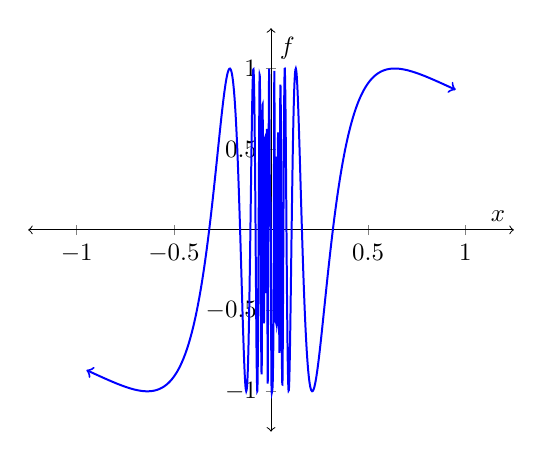
\begin{tikzpicture}[scale=0.9]
                \begin{axis}[
                	axis x line=middle,
                	xmax=1.25, xmin=-1.25,
                	axis y line=center,
                	ymax=1.25, ymin=-1.25,
                	xlabel=$x$,ylabel=$f$,
                	axis line style=<->
                    ]
                    \addplot[name path=f,smooth,domain=-0.95:0.95,color=blue,samples=500,thick,<->,] {sin(deg(1/x)};
                \end{axis}
            \end{tikzpicture}
        \end{center}
        
Here we would say that $\disp\lim_{x\to 0}\sin\lp\disp\frac{1}{x}\rp$ does not exist (DNE). We will not encounter many functions that behave this way in our course.

\vspace{5mm}

\textbf{One-Sided Limits.}

\vspace{3mm}

\boxenv{Definition.}{The limit of $f$ as $x$ approaches $c$ \textbf{from the left} is written as 

\vspace{15mm}

and is read ``the limit of $f$ as $x$ approaches $c$ from the left is $L$.''}

\vspace{3mm}

\boxenv{Definition.}{The limit of $f$ as $x$ approaches $c$ \textbf{from the right} is written as 

\vspace{15mm}

and is read ``the limit of $f$ as $x$ approaches $c$ from the right is $L$.''}

\vspace{5mm}

\boxenv{Remark.}{We interpret $x\to c^-$ to mean $x\to c$ and $x\to c^+$ to mean $x>c$.}

\vspace{3mm}

\boxenv{Theorem.}{Suppose $L\in\R$. We say that $\disp\lim_{x\to c}f(x)=L$ if and only if the one-sided limits exist and are equal. In other words\dots

\vspace{15mm}

Otherwise, we say that $\disp\lim_{x\to c}f(x)$ does not exist (DNE).}

\vspace{3mm}

We can now also say that a limit will not exist \textbf{at an endpoint} because an endpoint will not have both left and right limits.

\newpage 

Limits are not affected by what happens at a particular value. For $f(x)=\disp\frac{x^2-9}{x-3}$,
$$f(3)\text{ is undefined, but }\lim_{x\to 3}\frac{x^2-9}{x-3}=6.$$
Informally, a limit is more interested in the ``journey'' of a function than the ``destination.''

\vspace{3mm}

\Example Use the table of values to make a conjecture about $\disp\lim_{x\to 2}\frac{x^2-4}{x-2}$.

\vspace{5mm}

%\begin{center}
\renewcommand{\arraystretch}{2}
\begin{tabular}{ccccc}
\hline
\multicolumn{1}{|c|}{\cellcolor[HTML]{CBCEFB}$x$}    & \multicolumn{1}{c|}{1.9} & \multicolumn{1}{c|}{1.99} & \multicolumn{1}{c|}{1.999} & \multicolumn{1}{c|}{1.9999} \\ \hline
\multicolumn{1}{|c|}{\cellcolor[HTML]{CBCEFB}$\disp\frac{x^2-4}{x-2}$} & \multicolumn{1}{c|}{3.9} & \multicolumn{1}{c|}{3.99} & \multicolumn{1}{c|}{3.999} & \multicolumn{1}{c|}{3.9999} \\ \hline
\multicolumn{1}{l}{}                               & \multicolumn{1}{l}{}     & \multicolumn{1}{l}{}      & \multicolumn{1}{l}{}       & \multicolumn{1}{l}{}        \\ \hline
\multicolumn{1}{|c|}{\cellcolor[HTML]{CBCEFB}$x$}    & \multicolumn{1}{c|}{2.1} & \multicolumn{1}{c|}{2.01} & \multicolumn{1}{c|}{2.001} & \multicolumn{1}{c|}{2.0001} \\ \hline
\multicolumn{1}{|c|}{\cellcolor[HTML]{CBCEFB}$\disp\frac{x^2-4}{x-2}$} & \multicolumn{1}{c|}{4.1} & \multicolumn{1}{c|}{4.01} & \multicolumn{1}{c|}{4.001} & \multicolumn{1}{c|}{4.0001}  \\ \hline
\end{tabular}
%\end{center}

\vspace{10mm}

\textbf{Finding Limits Graphically.}

\vspace{5mm}

\begin{minipage}{.5\textwidth}
	\begin{center}
            \begin{tikzpicture}[scale=1]
                \begin{axis}[
                	axis x line=middle,
                	xmax=3.2, xmin=-3.2,
                	axis y line=center,
                	ymax=2.2, ymin=-2.2,
                	xlabel=$t$,ylabel=$f$,
                	axis line style=<->
                    ]
                    \addplot[name path=f,smooth,domain=-3:-2,color=blue,samples=100,thick,<-] {x+2};
                    \addplot[name path=f,smooth,domain=-2:-1,color=blue,samples=100,thick] {-x-2};
                    \addplot[name path=f,smooth,domain=-1:0,color=blue,samples=100,thick] {-1};
                    \addplot[name path=f,smooth,domain=0:3,color=blue,samples=100,thick,->] {1};	
		    \addplot[mark=*,color=blue] coordinates {(-2,0)};	
		    \addplot[mark=*,color=blue] coordinates {(0,0)};	
		    \addplot[mark=*,color=blue,fill=white] coordinates {(0,-1)};	
		    \addplot[mark=*,color=blue,fill=white] coordinates {(0,1)};	
                \end{axis}
            \end{tikzpicture}
        \end{center}
\end{minipage}%
\begin{minipage}{.5\textwidth}
	\begin{center}
            \begin{tikzpicture}[scale=1]
                \begin{axis}[
                	axis x line=middle,
                	xmax=4.2, xmin=-2.2,
                	axis y line=center,
                	ymax=3.2, ymin=-1.2,
                	xlabel=$x$,ylabel=$f$,
                	axis line style=<->
                    ]
                    \addplot[name path=f,smooth,domain=0:1,color=blue,samples=100,thick] {2*x^2};
                    \addplot[name path=f,smooth,domain=-1:0,color=blue,samples=100,thick] {-(x+1)^2+1};
                    \addplot[name path=f,smooth,domain=1:3,color=blue,samples=100,thick] {1};	
		    \addplot[mark=*,color=blue] coordinates {(-1,1)};	
		    \addplot[mark=*,color=blue] coordinates {(0,1)};	
		    \addplot[mark=*,color=blue] coordinates {(1,1)};
		    \addplot[mark=*,color=blue] coordinates {(3,1)};
		    \addplot[mark=*,color=blue] coordinates {(2,2)};			
		    \addplot[mark=*,color=blue,fill=white] coordinates {(1,2)};	
		    \addplot[mark=*,color=blue,fill=white] coordinates {(0,0)};
		    \addplot[mark=*,color=blue,fill=white] coordinates {(2,1)};		
                \end{axis}
            \end{tikzpicture}
        \end{center}
\end{minipage}


\end{document}